\begin{figure*}[hbtp]
  \centering
  \subfigure{
    \label{fig:louvain-compare--all}
    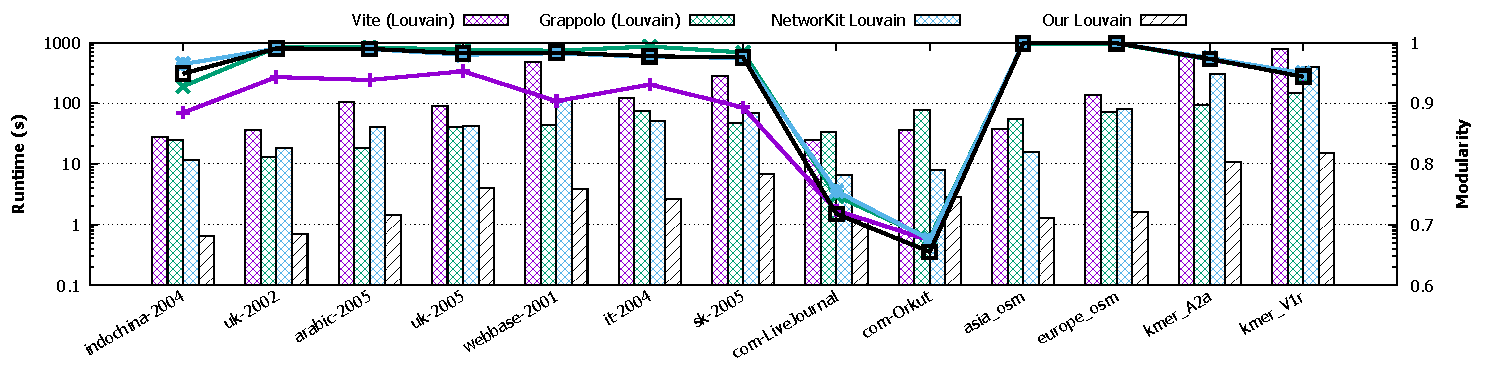
\includegraphics[width=0.98\linewidth]{out/louvain-compare.pdf}
  } \\[-2ex]
  \caption{Time taken (boxes), and modularity of communities obtained (lines) with \textit{Vite}, \textit{Grappolo}, \textit{NetworKit}, and our \textit{Louvain} for each graph in the dataset. Runtime is shown with logarithmic scale on the left Y-axis (in seconds), and modularity is shown with linear scale on the right Y-axis.}
  \label{fig:louvain-compare}
\end{figure*}
